Custom data types offer you the opportunity to define how data is organised in your program. You can create records that contain a number of fields, unions that store a single field value, and enumerations that define their own list of values. To help you understand these concepts better the following illustrations demonstrate how these values are stored in the variables in your code.

\subsection{Understanding \texttt{Read Row}} % (fold)
\label{ssub:understanding_read row}

\sref{sub:designing_small_db} \nameref{sub:designing_small_db} described the design of a Small DB program. The program allows the user to enter some values that were then stored in variables in the program, making use of records, unions, and enumerations. The design for this program included a number of functions and procedures, one of which was the \texttt{Read Row} function. This function was responsible for reading a row value from the user and returning it in a \texttt{Row} record. The flowchart for this function is shown in \fref{fig:read-row-flow-understanding}, which is a repeat of \fref{fig:read-row-flow}.

The following illustrations will show this code running to read in a value from the user. This will demonstrate how the computer stores values in record, union, and enumeration variables.

The illustrations will show the following:
\begin{enumerate}
  \item \nameref{ssub:code_is_loaded_for_small_db}
  \item \nameref{ssub:read_row_is_called_to_read_in_row_with_id_0}
  \item \nameref{ssub:step_1_stores_the_value_0_in_result_s_id_field}
  \item \nameref{ssub:a_double_value_is_entered_by_the_user}
  \item \nameref{ssub:the_double_data_is_stored_in_the_row}
  \item \nameref{ssub:the_result_row_is_returned_to_main}
  \item \nameref{ssub:this_process_is_repeated_for_each_element_of_the_array}
\end{enumerate}

\begin{figure}[p]
   \centering
   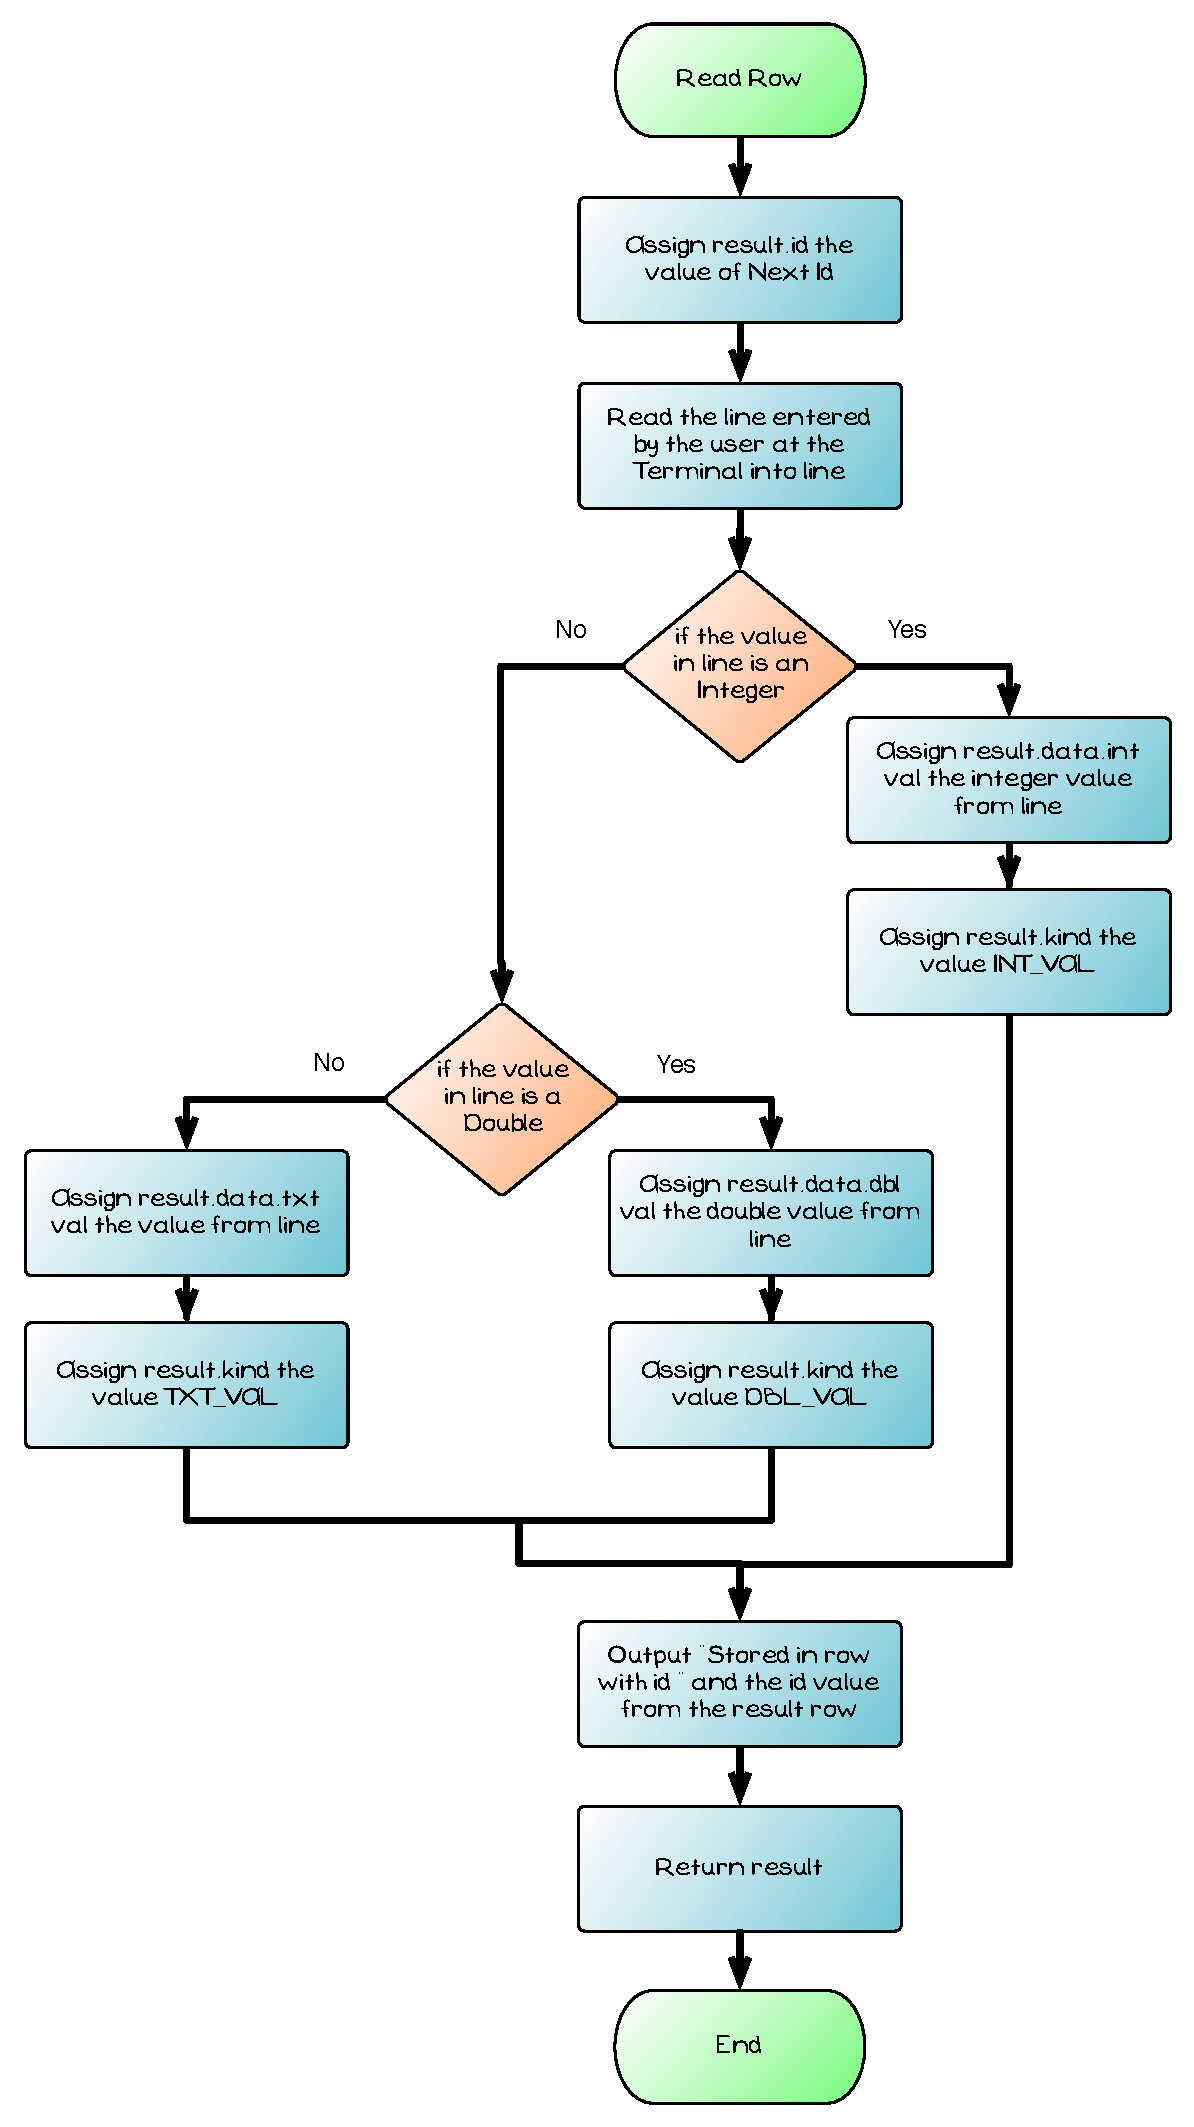
\includegraphics[width=0.80\textwidth]{./topics/type-decl/diagrams/ReadRowFlow} 
   \caption{Flowchart for \texttt{Read Row}, from \fref{fig:read-row-flow}}
   \label{fig:read-row-flow-understanding}
\end{figure}

\clearpage
\subsubsection{Code is loaded for Small DB} % (fold)
\label{ssub:code_is_loaded_for_small_db}

When the program starts its code is loaded into memory and its \texttt{main} procedure is started.

\begin{figure}[htbp]
   \centering
   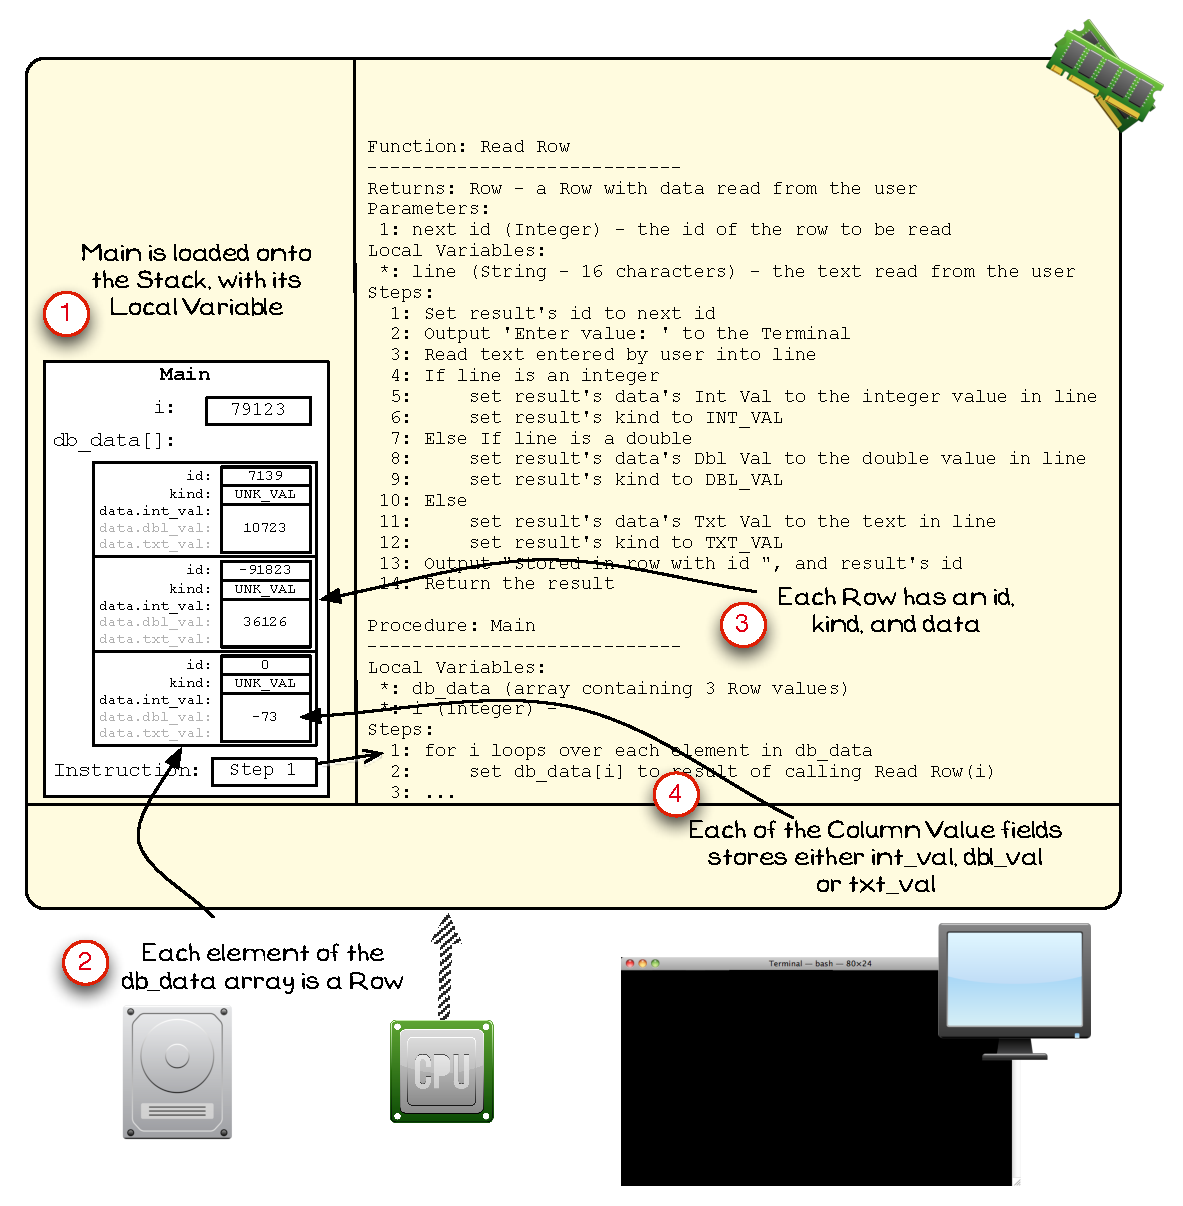
\includegraphics[width=0.9\textwidth]{./topics/type-decl/images/ReadRow1} 
   \caption{When the program starts \texttt{Main} allocates space for its local variables, including the array}
   \label{fig:read-row-vis-1}
\end{figure}

\mynote{
\begin{itemize}
  \item In \fref{fig:read-row-vis-1} the indicated areas show the following:
  \begin{enumerate}
    \item The Program starts and \texttt{Main} is loaded onto the stack, allocating space for its local variables.
    \item The \texttt{db\_data} array is allocated space to store its values. Each element of the array has the fields declared in the \texttt{Row} record structure.
    \item Each \texttt{Row} has an \texttt{id}, \texttt{kind}, and \texttt{data} value.
    \item Each of these \texttt{data} values has \emph{either} a \texttt{int\_val}, a \texttt{dbl\_val} or a \texttt{txt\_val}.
  \end{enumerate}
  \medskip
  \item Notice that the values in the array are allocated next to each other.
  \item In the illustration the \texttt{Row}'s \texttt{data} field will have only one of its fields highlighted, indicating which field is currently stored in the union.
\end{itemize}
}

% subsubsection code_is_loaded_for_small_db (end)

\clearpage
\subsubsection{\texttt{Read Row} is called to read in row with id 0} % (fold)
\label{ssub:read_row_is_called_to_read_in_row_with_id_0}

The \texttt{Read Row} function is called to read a \texttt{row} value from the user. This will check what the user has entered and store an appropriate value in the \texttt{Row} it returns.

\begin{figure}[htbp]
   \centering
   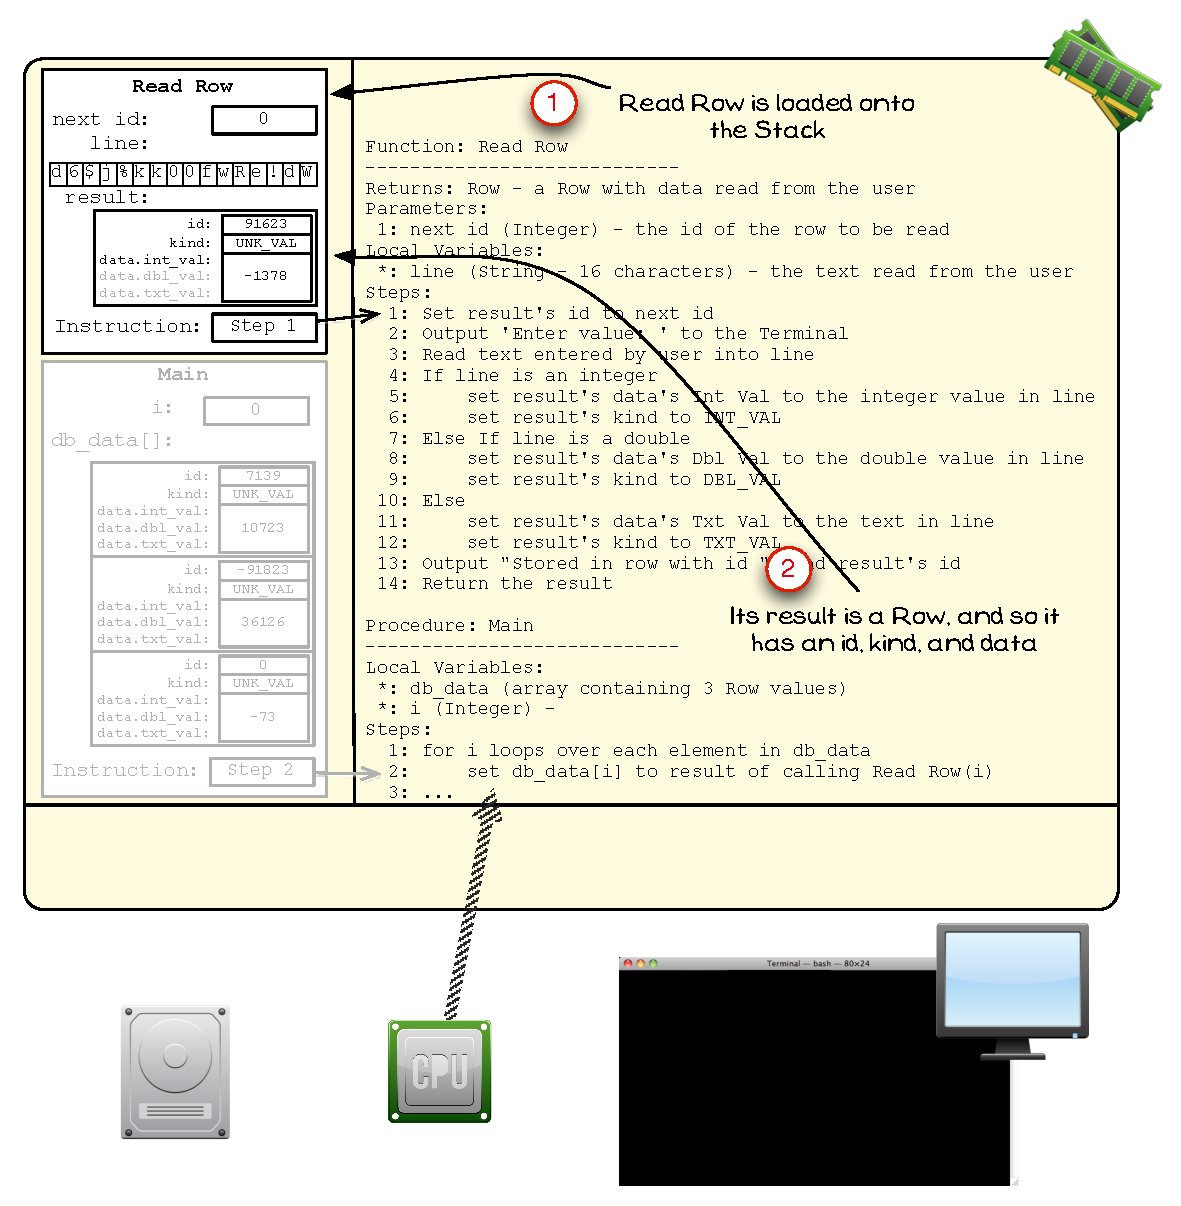
\includegraphics[width=\textwidth]{./topics/type-decl/images/ReadRow2} 
   \caption{At step 2 \texttt{Main} calls \texttt{Read Row}, getting it to read in the $i^{th}$ row from the user}
   \label{fig:read-row-vis-2}
\end{figure}

\mynote{
\begin{itemize}
  \item In \fref{fig:read-row-vis-2} the indicated areas show the following:
  \begin{enumerate}
    \item When \texttt{Read Row} is called it is allocated space on the stack.
    \item \texttt{Read Row} will be returning a \texttt{Row} value, so its result will have \texttt{id}, \texttt{kind}, and \texttt{data} values as these are what is specified in the \texttt{Row} record's definition.
  \end{enumerate}
  \medskip
  \item Each row will have the same kind of data stored within it. The details of this are specified in the \texttt{Row} record's definition.
\end{itemize}
}

% subsubsection read_row_is_called_to_read_in_row_with_id_0 (end)

\clearpage
\subsubsection{Step 1 stores the value 0 in \texttt{result}'s \texttt{id} field} % (fold)
\label{ssub:step_1_stores_the_value_0_in_result_s_id_field}

\begin{figure}[htbp]
   \centering
   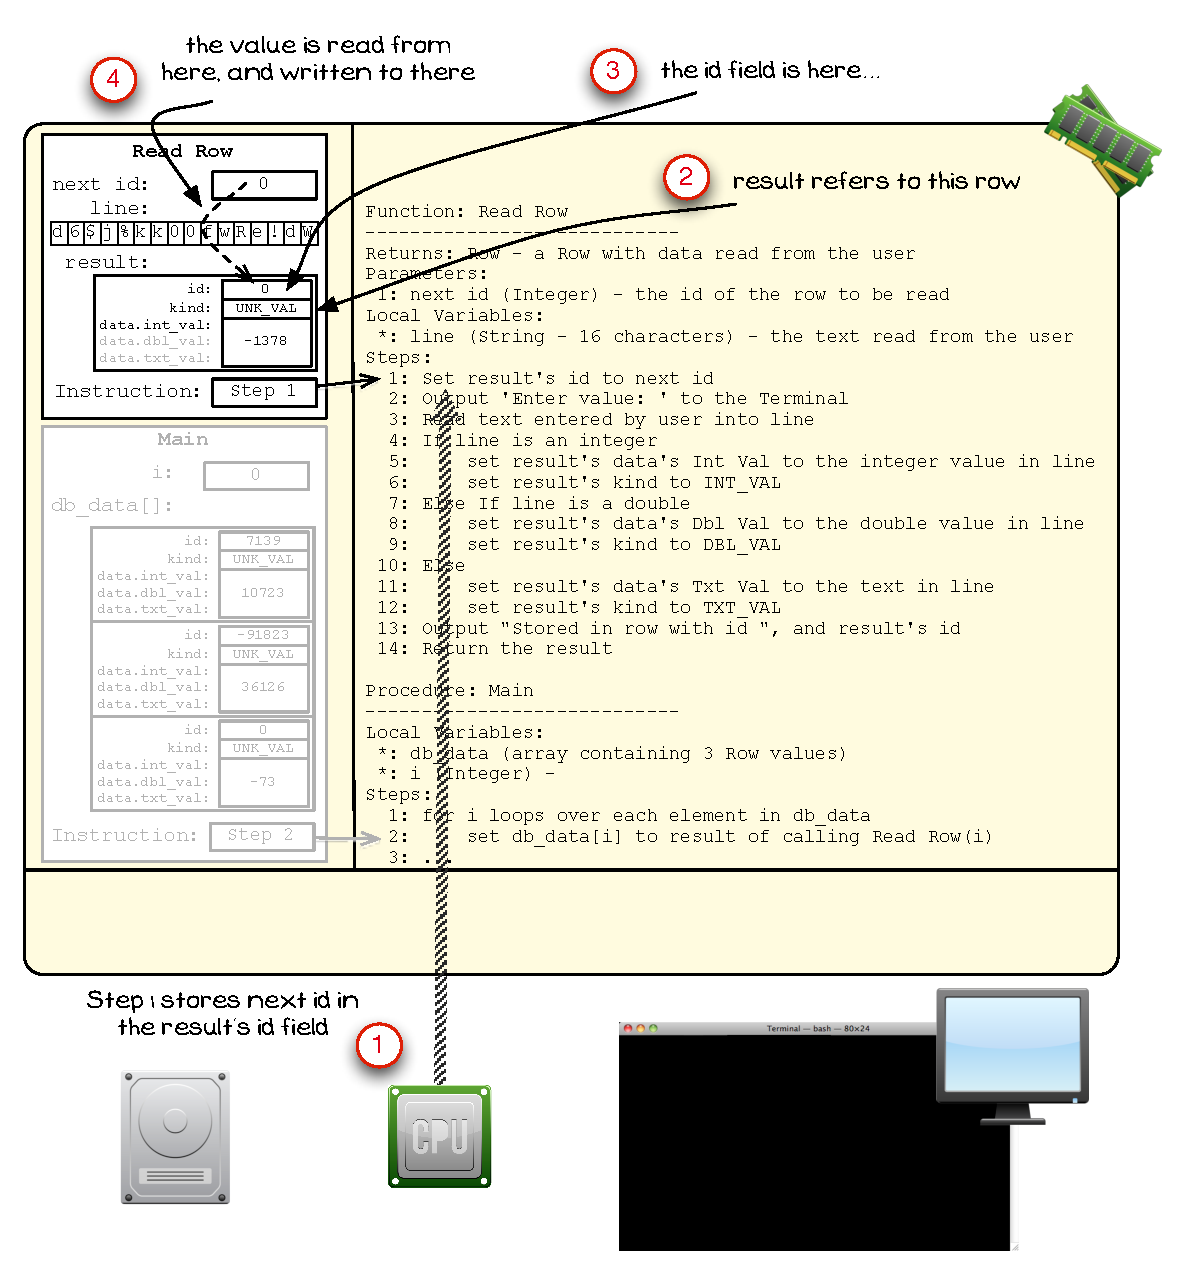
\includegraphics[width=0.98\textwidth]{./topics/type-decl/images/ReadRow3} 
 \caption{Step 1 of \texttt{Read Row} stores a value in \texttt{result}'s id}
 \label{fig:read-row-vis-3}
\end{figure}

\mynote{
\begin{itemize}
\item In \fref{fig:read-row-vis-3} the indicated areas show the following:
\begin{enumerate}
  \item Step 1 of \texttt{Read Row} assigns a value to \texttt{result.id}.
  \item In this code \texttt{result} refers to this variable in \texttt{Read Row}.
  \item The \texttt{id} part then refers to this field.
  \item As a result the value from the \texttt{next id} parameter is read, and its value is assigned to \texttt{result.id}.
\end{enumerate}
\medskip
\item Each part of \texttt{result.id} refers to a different kind of data.
\item \texttt{result} is a row, this has \texttt{id}, \texttt{kind}, and \texttt{data} fields.
\item \texttt{result.id} is an \texttt{Integer}, it is the id field of the \texttt{result Row}.
\end{itemize}
}

% subsubsection step_1_stores_a_value_in_result_s_id_field (end)

\clearpage
\subsubsection{A double value is entered by the user} % (fold)
\label{ssub:a_double_value_is_entered_by_the_user}

\begin{figure}[htbp]
   \centering
   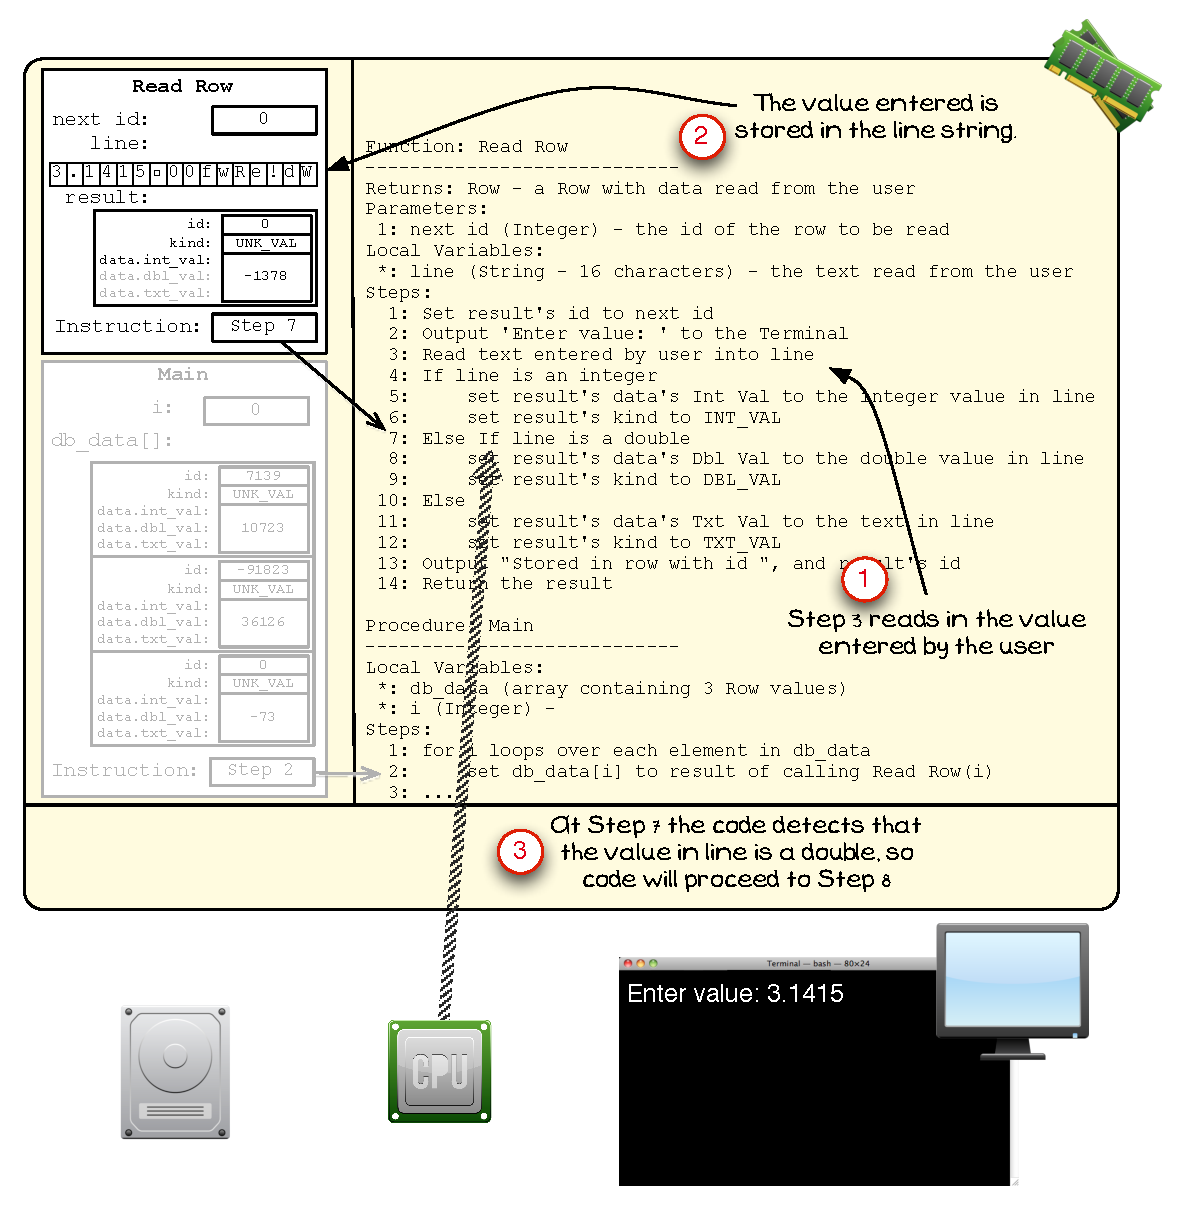
\includegraphics[width=0.98\textwidth]{./topics/type-decl/images/ReadRow4} 
 \caption{A double value is entered by the user, so the code must store the double in the row}
 \label{fig:read-row-vis-4}
\end{figure}

\mynote{
\begin{itemize}
\item In \fref{fig:read-row-vis-4} the indicated areas show the following:
\begin{enumerate}
  \item At Step 3 the computer reads the text entered by the user.
  \item The value read is stored in the \texttt{line} variable.
  \item At Step 7 the code determines that the data is a double, and execution will proceed to step 8.
\end{enumerate}
\medskip
\end{itemize}
}

% subsubsection a_double_value_is_entered_by_the_user (end)

\clearpage
\subsubsection{The double data is stored in the row} % (fold)
\label{ssub:the_double_data_is_stored_in_the_row}

\begin{figure}[htbp]
   \centering
   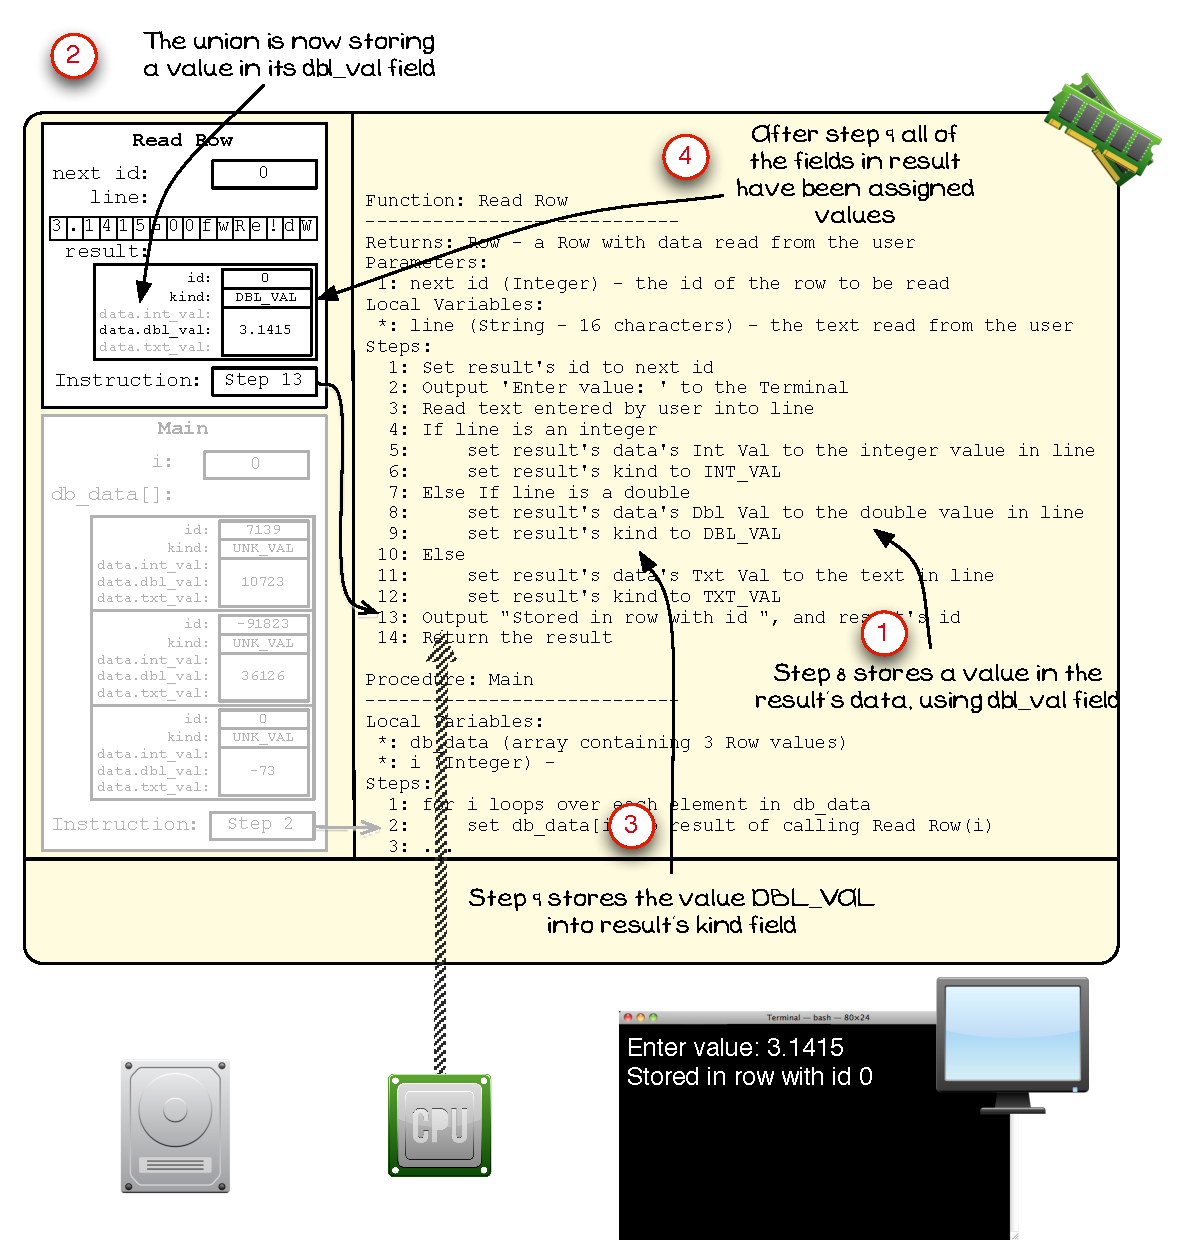
\includegraphics[width=\textwidth]{./topics/type-decl/images/ReadRow5} 
 \caption{A double value is entered by the user, so the code must store the double in the row}
 \label{fig:read-row-vis-5}
\end{figure}

\mynote{
\begin{itemize}
\item In \fref{fig:read-row-vis-5} the indicated areas show the following:
\begin{enumerate}
  \item Step 8 of \texttt{Read Row} stores the double value entered by the user into the \texttt{dbl\_val} field of the \texttt{data} field of the \texttt{result Row}.
  \item Notice that the union is now shown as storing a value in its \texttt{dbl\_val} field.
  \item Step 9 stores the \texttt{DBL\_VAL} value in the \texttt{kind} field of the \texttt{result Row}. This is one of the values from the \texttt{Data Kind} enumeration.
  \item At this point all of the fields of \texttt{result} have been assigned values.
\end{enumerate}
\medskip
\end{itemize}
}

% subsubsection the_double_data_is_stored_in_the_row (end)

\clearpage
\subsubsection{The \texttt{result} row is returned to \texttt{Main}} % (fold)
\label{ssub:the_result_row_is_returned_to_main}

\begin{figure}[htbp]
   \centering
   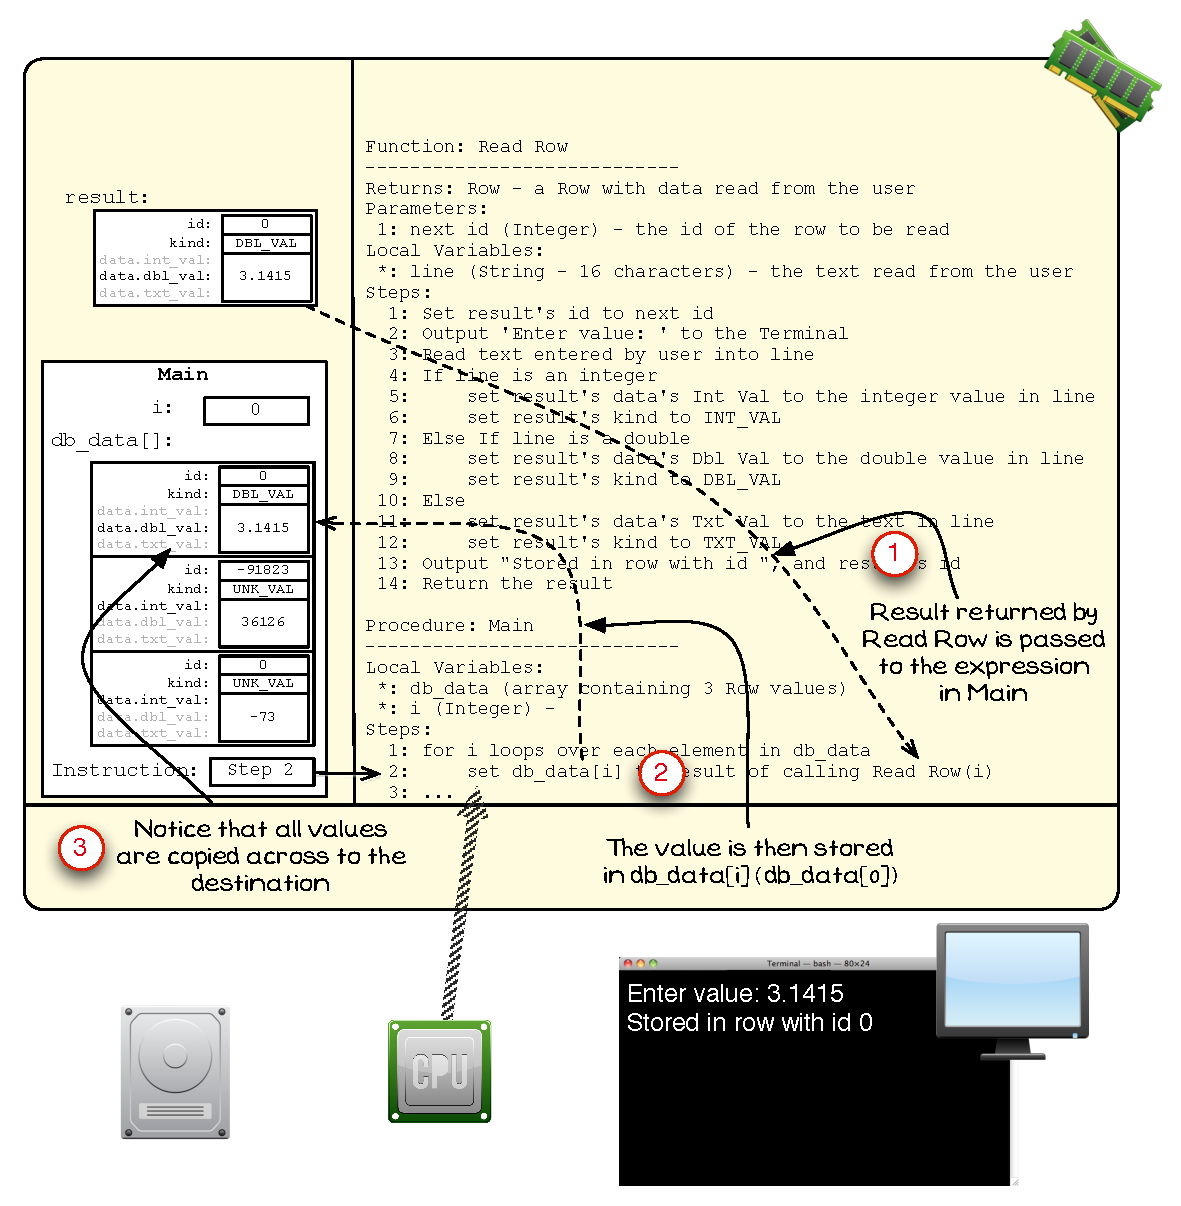
\includegraphics[width=\textwidth]{./topics/type-decl/images/ReadRow6} 
 \caption{The \texttt{result Row} is returned to \texttt{Main}}
 \label{fig:read-row-vis-6}
\end{figure}

\mynote{
\begin{itemize}
\item In \fref{fig:read-row-vis-6} the indicated areas show the following:
\begin{enumerate}
  \item At the end of \texttt{Read Row} the \texttt{result Row} is returned to \texttt{Main}.
  \item In \texttt{Main} the value is used in an assignment statement, that assigns it to the $i^{th}$ value in the \texttt{db\_data} array. As \texttt{i} is currently 0, this stores the \textbf{entire} row in \texttt{dd\_data[0]}.
  \item When this assignment occurs all of the data from the \texttt{result} of \texttt{Read Row} is copied into \texttt{db\_data[0]}.
\end{enumerate}
\medskip
\item With Records and Unions you can read/write to individual fields using the dot notation, or you can access the entire record.
\end{itemize}
}


% subsubsection the_result_row_is_returned_to_main (end)

\clearpage
\subsubsection{This process is repeated for each element of the array} % (fold)
\label{ssub:this_process_is_repeated_for_each_element_of_the_array}

\begin{figure}[htbp]
   \centering
   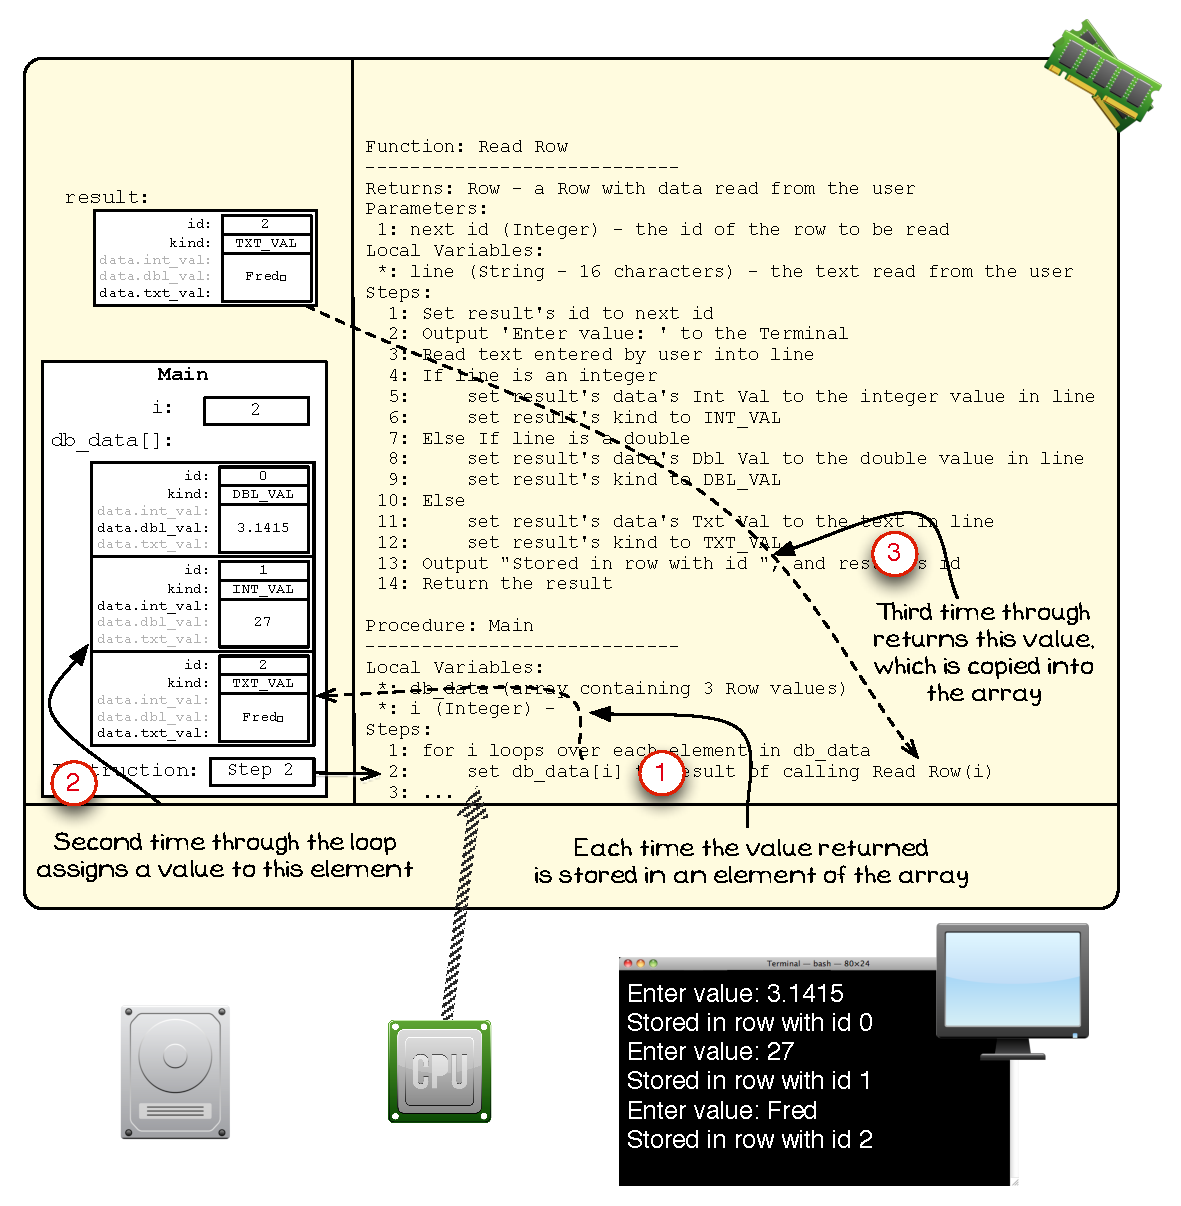
\includegraphics[width=0.92\textwidth]{./topics/type-decl/images/ReadRow7} 
 \caption{The for loop ensures that a \texttt{Row} value is read in for each element of the array}
 \label{fig:read-row-vis-7}
\end{figure}

\mynote{
\begin{itemize}
\item In \fref{fig:read-row-vis-7} the indicated areas show the following:
\begin{enumerate}
  \item Each time through the loop the value is written to an element in the array. This is showing the last iteration where \texttt{i} is 2.
  \item The second time this loop was executed the user entered an integer value, this is now stored in the second element of the array.
  \item The third time through the loop, the result returned is storing a string value. This is returned to \texttt{Main}, and then stored in the \texttt{db\_data} array.
\end{enumerate}
\medskip
\item Notice that there is only ever one value in each \texttt{Row}'s \texttt{data}. This is a \textbf{union}, and only stores one of its field values.
\item See how the enumeration values indicate the field the data has been stored in. This is why the enumeration's constants were named in a similar\footnote{They could have been named anything, but this reflects their purpose well.} way to the union's fields.
\end{itemize}
}

% subsubsection this_process_is_repeated_for_each_element_of_the_array (end)

% subsection understanding_read row (end)
\clearpage
\subsection{Understanding \texttt{Print Row}} % (fold)
\label{sub:understanding_print row}

\texttt{Print Row} is the other key piece of logic in the Small DB program. This procedure outputs the values read from the user to the Terminal. It uses the data stored in the \texttt{Row}'s fields to determine how this value is output, and how the data can be read. The flowchart of this logic is shown in \fref{fig:print-row-flow-understanding}.

\begin{figure}[htbp]
   \centering
   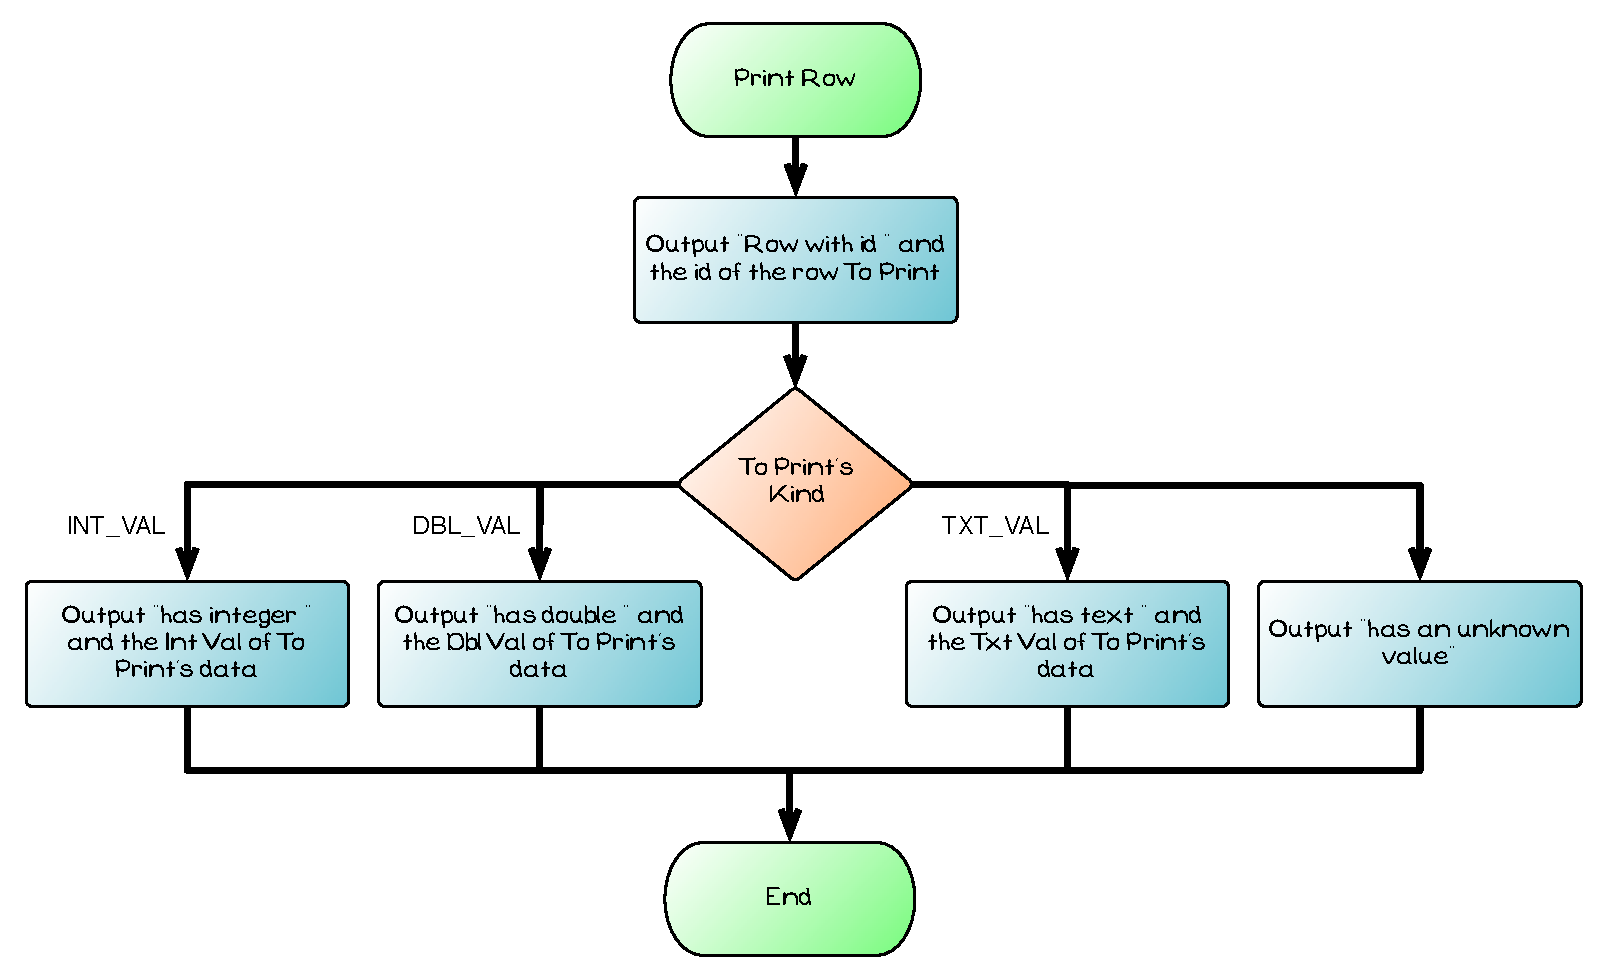
\includegraphics[width=\textwidth]{./topics/type-decl/diagrams/PrintRowFlow} 
   \caption{Flowchart of the steps needed to print a \texttt{Row} to the Terminal, from \fref{fig:print-row-flow}}
   \label{fig:print-row-flow-understanding}
\end{figure}

Within \texttt{Main}, \texttt{Print Row} is called once for each \texttt{Row} in the \texttt{db\_data} array. The following illustrations demonstrate the third and final call to \texttt{Print Row}.

The illustrations will show the following:
\begin{enumerate}
  \item \nameref{ssub:print_row_is_called_for_each_element_in_the_array}
  \item \nameref{ssub:the_text_value_is_output_to_the_terminal}
\end{enumerate}

You can use these details to determine how the other data was written to the Terminal. 

\clearpage
\subsubsection{\texttt{Print Row} is called for each element in the array} % (fold)
\label{ssub:print_row_is_called_for_each_element_in_the_array}

This illustration starts part way through the third call to \texttt{Print Row}. At this stage the first two rows have been output to the Terminal, as has the \texttt{id} of the third \texttt{Row}.

\begin{figure}[htbp]
   \centering
   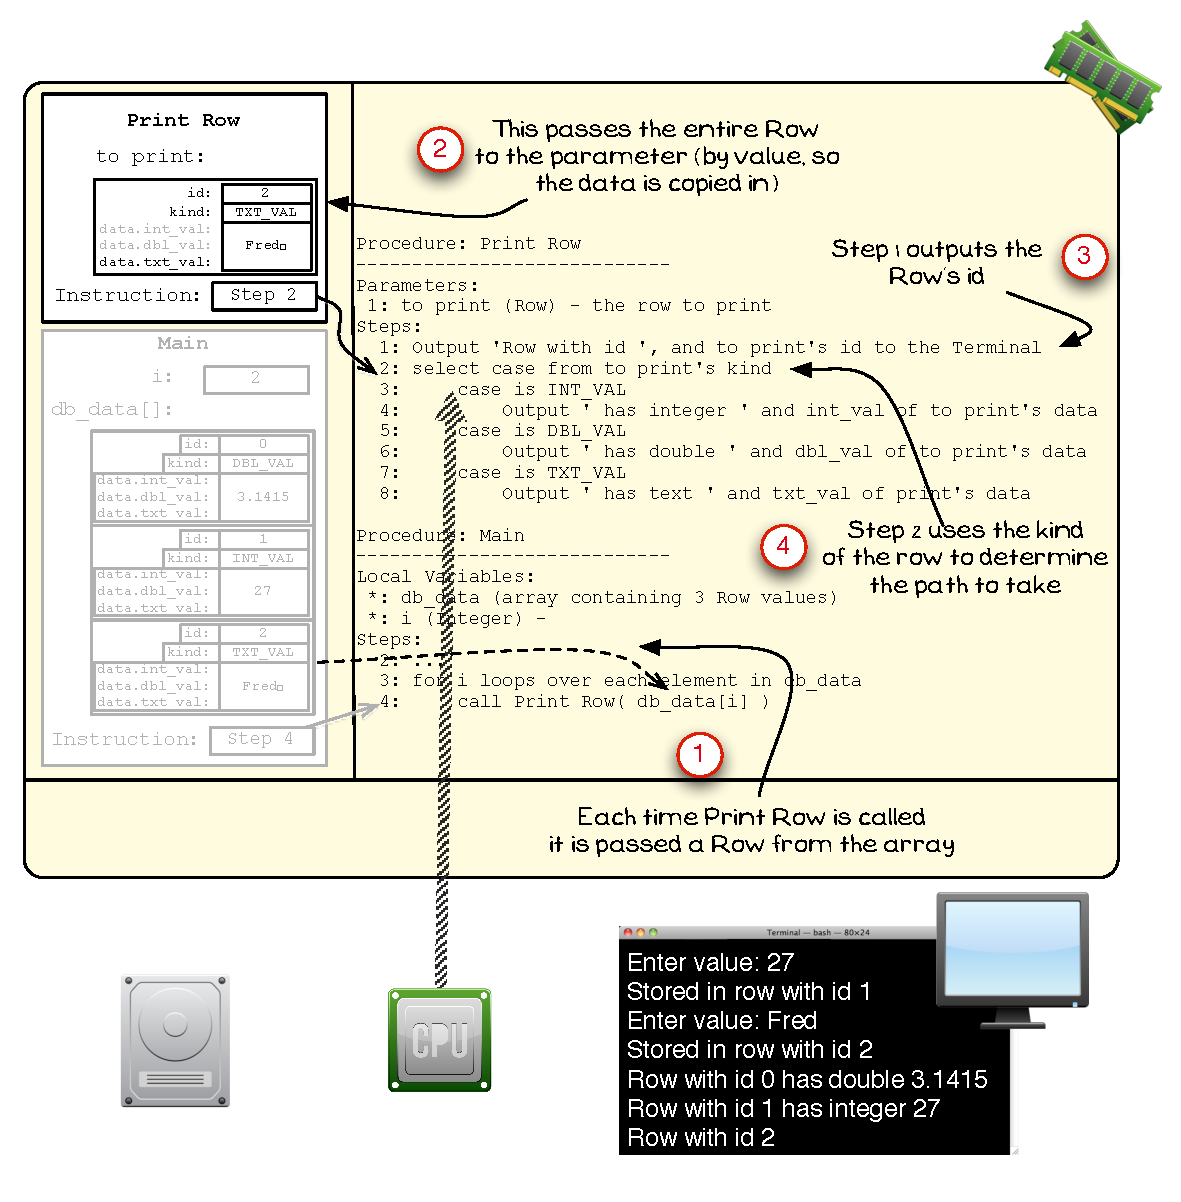
\includegraphics[width=0.92\textwidth]{./topics/type-decl/images/PrintRow1} 
 \caption{\texttt{Print Row} is called for each of the \texttt{Row} elements in \texttt{db\_data}}
 \label{fig:print-row-vis-1}
\end{figure}

\mynote{
\begin{itemize}
\item In \fref{fig:print-row-vis-1} the indicated areas show the following:
\begin{enumerate}
  \item This is the third call to \texttt{Print Row}. Each time this procedure is called it receives a copy of the data from the element passed to it.
  \item The parameter is a copy of the data from the array element.
  \item The first action in \texttt{Print Row} is to output the \texttt{id} value from the \texttt{to print} \texttt{Row}.
  \item The illustration is showing the computer at the stage where it is reading \texttt{to print}'s \texttt{kind} to determine which path to take. As \texttt{to print}'s \texttt{kind} is currently \texttt{TXT\_VAL} it will take the path at Step 8.
\end{enumerate}
\medskip
\item The case statement will allow the code to output the message that matches the kind of data stored in \texttt{to print}.
\end{itemize}
}

% subsubsection print_row_is_called_for_each_element_in_the_array (end)

\clearpage
\subsubsection{The text value is output to the Terminal} % (fold)
\label{ssub:the_text_value_is_output_to_the_terminal}

\begin{figure}[htbp]
   \centering
   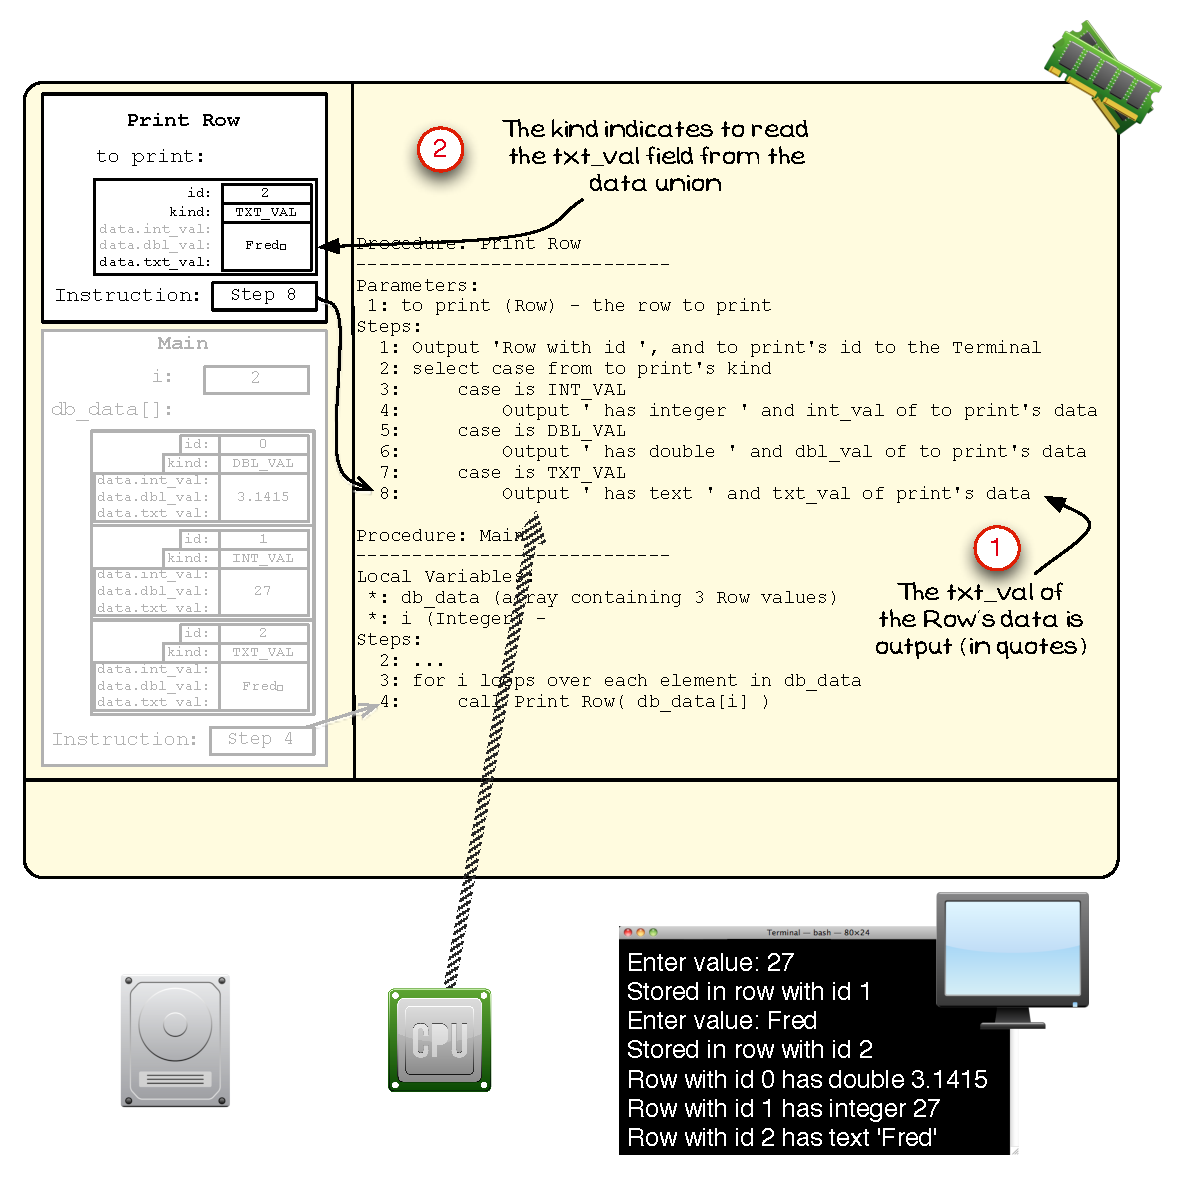
\includegraphics[width=0.91\textwidth]{./topics/type-decl/images/PrintRow2} 
 \caption{\texttt{Print Row} is called for each of the \texttt{Row} elements in \texttt{db\_data}}
 \label{fig:print-row-vis-2}
\end{figure}

\mynote{
\begin{itemize}
\item In \fref{fig:print-row-vis-2} the indicated areas show the following:
\begin{enumerate}
  \item Step 8 reads the \texttt{txt\_val} field of \texttt{to print}'s \texttt{data} field. This reads the text value from within that field, and this is output to the Terminal.
  \item The \texttt{kind} field was used to determine which field to read from the union.
\end{enumerate}
\smallskip
\item In this example the record, union, and enumeration are all working together to enable the required functionality.
\item Without the enumeration it would not be possible to determine which field to read from the union. Reading any of the fields on the union would return data, but only the field that was written to can be relied about to have a meaningful value.
\item Without the union you would need to waste space storing all three data values, but only ever using one.
\item Without the record it would be hard to relate the values stored within a single \texttt{Row}. The row only existed because of the record's declaration.
\item Back in \texttt{Main}, the array allows you to store multiple of these values. 
\end{itemize}
}


% subsubsection the_text_value_is_output_to_the_terminal (end)


% subsection understanding_print row (end)